\documentclass[xcolor=dvipsnames, aspectratio = 169]{beamer}
\usepackage[english]{babel} %% english
\usepackage[utf8]{inputenc}
\usepackage[T1]{fontenc}
\usepackage{include/chariteBeamer}
\usepackage{hyperref}
\author[E. Sprünken]{Erin Sprünken}
\institute[]{
Institut für Biometrie und Klinische Epidemiologie\\[1Ex] 
Charité - Universitätsmedizin Berlin, Berlin\\[1Ex]
erin-dirk.spruenken@charite.de} 
\titlegraphic{\pgfuseimage{frontUnilogo}}

\tikzset{>=latex}
%\usepackage{amsmath}
%\usetikzlibrary{shadows}
\usepackage[edges]{forest}
\usetikzlibrary{positioning}
\usepackage{biostat}
\setbeamertemplate{caption}[numbered]
\let\qed\relax
\forestset{declare toks={elo}{}}
%% ================================================================== %% 

\author[L. Mödl, M. Becher, E. Sprünken]{Lukas Mödl, Matthias Becher, Erin Sprünken} 
\title{R-Kurs: Tag 2} 
\date[]{\today}

%% ================================================================== %% 
\setbeamercolor*{mycol}{bg=chariteGray, fg=chariteBlue}

\hyphenation{Sam-ples}
\begin{document}

%% ================================================================== %%
%% ================================================================== %%
\setbeamertemplate{footline}{\begin{tikzpicture}
    \node [inner sep=0pt, anchor=east] (0,0) {
      
\includegraphics[width=\paperwidth,height=0.7cm]{include/charite_footer}};
    \node [inner sep=0pt, anchor=east] at (-0.5ex,-0ex){};
\end{tikzpicture}}

\setbeamertemplate{headline}{
%\leavevmode
\hspace{-0.49em}\hbox{
	\begin{beamercolorbox}[wd=1.02\paperwidth,ht=2.25ex,dp=1ex,left]{mycol}%
    \usebeamerfont{section in head/foot}
  \end{beamercolorbox}%
}}
{
  \usebackgroundtemplate{ \hspace{-0.5em}\begin{tikzpicture}
  \node[opacity=0.7, anchor=south] (0,0) {
\includegraphics[height=\paperheight, width=1.04\paperwidth]{include/frontmatter.pdf}};
  \end{tikzpicture}
} 
%\frame{\titlepage}
\begin{frame}
\centering
	\vspace{4em}
	{\Large \textcolor{chariteBlue}{\inserttitle}}\\
	 \vspace{1em}
	{\Large \textcolor{black}{\insertauthor \\}} 
	\vspace{2em}
	{\footnotesize \textcolor{black}{\insertinstitute \\\vspace{1em} \insertdate}} 
	\vspace{0em}
	\begin{figure}[h!]
		
\includegraphics[width=5cm]{include/Charite_Logo.png}
	\end{figure}
%	\pgfuseimage{frontUnilogo}
\end{frame}
}
%% ================================================================== %%

\setbeamertemplate{footline}{\begin{tikzpicture}
    \node [inner sep=0pt, anchor=east] (0,0) {
      
\includegraphics[width=\paperwidth,height=0.7cm]{include/charite_footer}};
    \node [inner sep=0pt, anchor=east] at (-0.5ex,-0ex) {\tiny \insertframenumber{}$\,$|$\,$\inserttotalframenumber};
\end{tikzpicture}}

\setbeamertemplate{headline}{%
%\leavevmode%
\hspace{-0.49em}\hbox{
	\begin{beamercolorbox}[wd=.68\paperwidth,ht=2.25ex,dp=1ex,left]{mycol}%
    \usebeamerfont{section in head/foot}\hspace*{1em}
  \end{beamercolorbox}%
  \begin{beamercolorbox}[wd=.20\paperwidth,ht=2.25ex,dp=1ex,right]{mycol}%
    \usebeamerfont{author in head/foot}\insertshortauthor
  \end{beamercolorbox}%
  \begin{beamercolorbox}[wd=.14\paperwidth,ht=2.25ex,dp=1ex,center]{mycol}%
    \usebeamerfont{date in head/foot}\insertdate
  \end{beamercolorbox}%
  }
}


\frame{\tableofcontents}

\setbeamertemplate{headline}{%
%\leavevmode%
\hspace{-0.49em}\hbox{
	\begin{beamercolorbox}[wd=.68\paperwidth,ht=2.25ex,dp=1ex,left]{mycol}%
    \usebeamerfont{section in head/foot}\hspace*{1em}\thesection. \  \insertsectionhead
  \end{beamercolorbox}%
  \begin{beamercolorbox}[wd=.20\paperwidth,ht=2.25ex,dp=1ex,right]{mycol}%
    \usebeamerfont{author in head/foot}\insertshortauthor
  \end{beamercolorbox}%
  \begin{beamercolorbox}[wd=.14\paperwidth,ht=2.25ex,dp=1ex,center]{mycol}%
    \usebeamerfont{date in head/foot}\insertdate
  \end{beamercolorbox}%
  }
}

\section{Laden von Daten}
\begin{frame}[fragile]{Laden}
  \begin{itemize}
	  \item \verb + load() +
	  \item  \verb + read.table() +
	  \item  \verb + read.csv() +
  \end{itemize}
\end{frame}

\begin{frame}[fragile]{Optionen bei read.csv()}
Wenn man CSVs in R lädt kann man verschiedene Parameter einstellen, um der Funktion zu sagen wie die CSV formatiert ist. Die wichtigsten werden hier vorgestellt:
  \begin{itemize}
	  \item \verb +header(TRUE/FALSE):+ Zeigt an ob in der CSV Spaltenname in der ersten Reihe stehen
	  \item \verb +sep:+Welches Zeichen wird verwendet um Spalten zu trennen. Default ist ",". Es werden aber auch häufig ";" oder "\textbackslash t" verwendet
	  \item \verb +dec:+Welches Zeichen wird bei Dezimalzahlen verwendet "." oder ","
	  \item	Beispiel: \verb +read.csv("data.csv", header=TRUE, sep=";", dec=",")+
  \end{itemize}
\end{frame}

%% ================================================================== %%
\section{Deskreptive Statistik}

\begin{frame}{Summary()}
	\begin{center}
		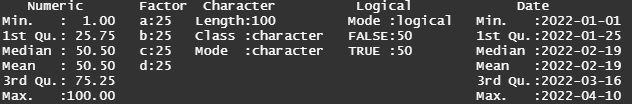
\includegraphics{Summary}
	\end{center}
\end{frame}

\begin{frame}[fragile]{Funktionen für die Deskreptive Statistik}
\begin{columns}[T]
	\begin{column}{0.5\textwidth}
		\begin{itemize}
			\item Mean = \verb+ mean() +
			\item Median = \verb+ median() +
			\item Minimum = \verb+ min() +
			\item Maximum = \verb+ max() +
			\item Standard Deviation = \verb+ sd() +
		\end{itemize}
	\end{column}
	\begin{column}{0.5\textwidth}
		\begin{itemize}
			\item Variance = \verb+ var() +
			\item Quantile = \verb+ quantile() +
			\item Correlation = \verb+ cor() +
			\item Covariance = \verb+ cov() +
			\item Crosstable = \verb+ table() +
		\end{itemize}
	\end{column}
\end{columns}
\end{frame}


%% ================================================================== %%
\section{Datenaufbereitung, Kovertierung und Verwendung}
\begin{frame}[fragile]{Konvertieren von Daten}
	\begin{itemize}
		\item Numeric $\Leftrightarrow$ \verb+as.numeric()+
		\item Character $\Leftrightarrow$ \verb+as.character()+
		\item Factor $\Leftrightarrow$ \verb+as.factor()+
		\item Date $\Leftrightarrow$ \verb+as.Date()+
		\item Logical $\Leftrightarrow$ \verb+as.logical()+
	\end{itemize}
\end{frame}

\begin{frame}[fragile]{Indiziereung}
	Häufig möchte man nur bestimmte Elemente eines Vektors, einer Liste oder eines Data Frames auswählen. Um das zu tun gibt es mehrere Möglichkeiten. Die direkteste ist es, die Indizes zu verwenden. Angenommen wir haben den Vektor \verb + x <- c(1, 2, 3, 4, 5) +
	\begin{itemize}
		\item  Einen bestimmten Wert auswählen $\Leftrightarrow$ \verb+ x[1]+
		\item  Mehrere Werte auswählen $\Leftrightarrow$\verb+ x[c(1, 3, 5)]+
		\item  Eine Reihe von Werten auswählen $\Leftrightarrow$\verb+ x[1:3]+
		\item  Einen bestimmten Wert weglassen $\Leftrightarrow$ \verb+x[-1]+
	\end{itemize}
\end{frame}

\begin{frame}[fragile]{Indiziereung von Listen und Data Frames}
	
	\begin{columns}[T]
	\begin{column}{0.5\textwidth}
Liste
		\begin{itemize}
		\item \verb+x[1]+
		\item \verb+x[[1]]+
		\item \verb+x[[1]][1]+
	\end{itemize}
	\end{column}
	\begin{column}{0.5\textwidth}
Data Frame
	\begin{itemize}
		\item  \verb+x[1,]+
		\item  \verb+x[,1]+
		\item  \verb+x[,"Spalte1" ]+
		\item  \verb+x$Spalte1+
	\end{itemize}
	\end{column}
\end{columns}

\end{frame}

\begin{frame}[fragile]{Filtern}
Häufig kommt es vor, dass wir unsere Daten filtern möchten um bespielsweise nur die Männer bzw. Frauen zu untersuchen oder nur Patiente ab einem bestimmten Alter zu betrachten. In R gibt es verschiedene Befehle mit denen man das erreichen kann.
	\begin{itemize}
		\item  \verb+which()+
		\begin{itemize}
			\item  \verb+data[which(data$Sex == "M"),]+
		\end{itemize}
		\item  \verb+%in%+
		\begin{itemize}
			\item  \verb+data[which(data$Color %in% c("blue", "red"),]+
		\end{itemize}
		\item  \verb+subset()+
		\begin{itemize}
			\item  \verb+subset(data, Age < 50,)+
		\end{itemize}
	\end{itemize}
\end{frame}

\begin{frame}[fragile]{Nach mehreren Sachen gleichzeitig Filtern}
Manchmal möchte man nach mehreren Spalten gleichzeitig filtern. Anstatt das nacheinaner zu tun, kann man auch mehrere Filter mit "\&" verbinden. \\
Zum Beispiel:
	\begin{itemize}
		\item  \verb+data[which(data$Sex == "W" & data$Age > 50),]+
	\end{itemize}
\end{frame}

%% ================================================================== %%

\section{Plots}

\begin{frame}[fragile]{Scatterplot}
	\begin{itemize}
		\item \verb+ plot(data$Spalte1, data$Spalte2)+
	\end{itemize}
			
	\begin{center}
		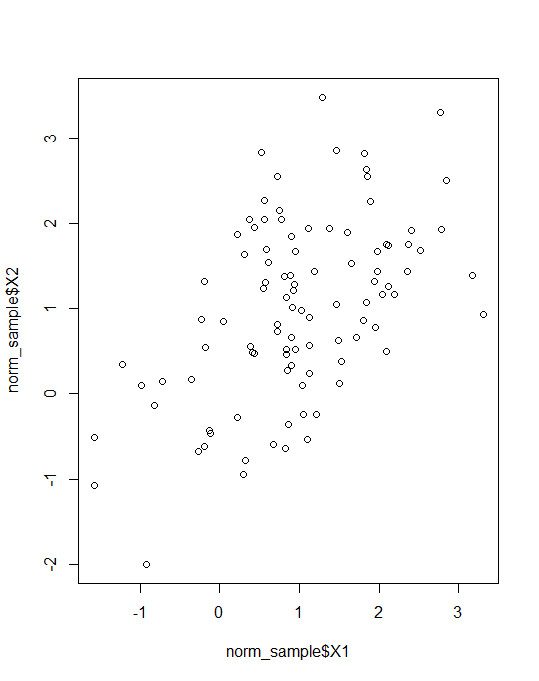
\includegraphics[height=6cm]{Scatterplot}
	\end{center}
\end{frame}

\begin{frame}[fragile]{Boxplot}
	\begin{itemize}
		\item \verb+boxplot(Spalte1 ~ Spalte2, data)+
	\end{itemize}
			
	\begin{center}
		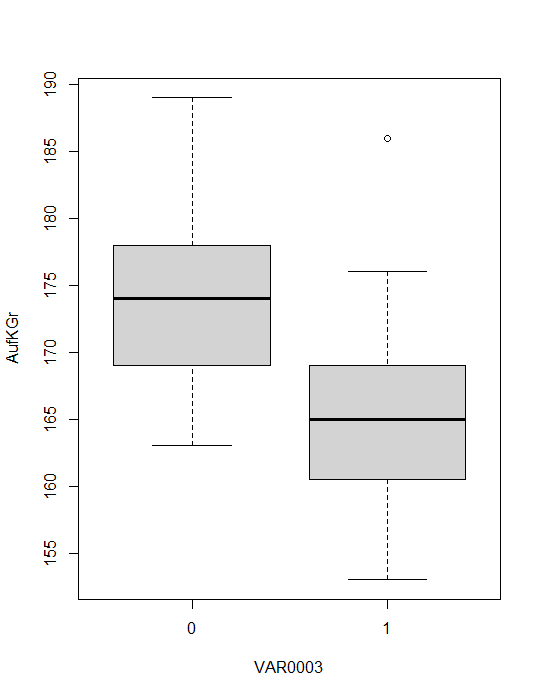
\includegraphics[height=6.5cm]{Boxplot}
	\end{center}
\end{frame}

\begin{frame}[fragile]{Histogram}
	\begin{itemize}
		\item \verb+hist(norm_sample$X1) +
	\end{itemize}
			
	\begin{center}
		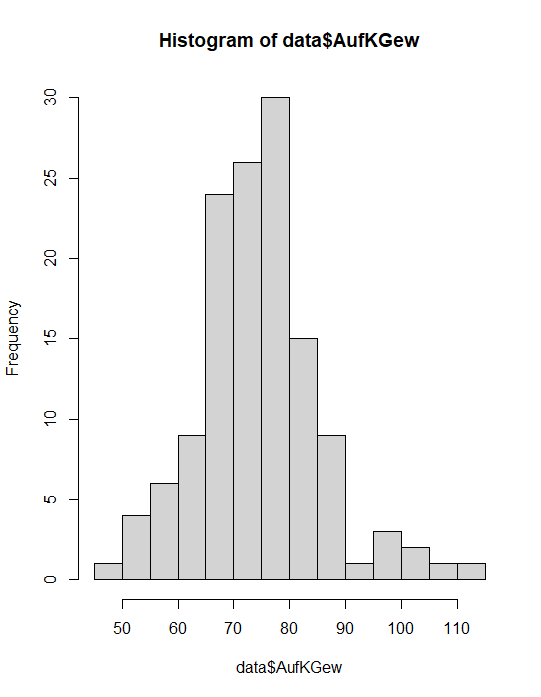
\includegraphics[height=6.5cm]{Histogram}
	\end{center}
\end{frame}

\begin{frame}[fragile]{Histogram mit Density}
	\begin{itemize}
		\item \verb+ hist(norm_sample$X1, probability = T)+ \\ \verb + lines(density(norm_sample$X1))+
	\end{itemize}
			
	\begin{center}
		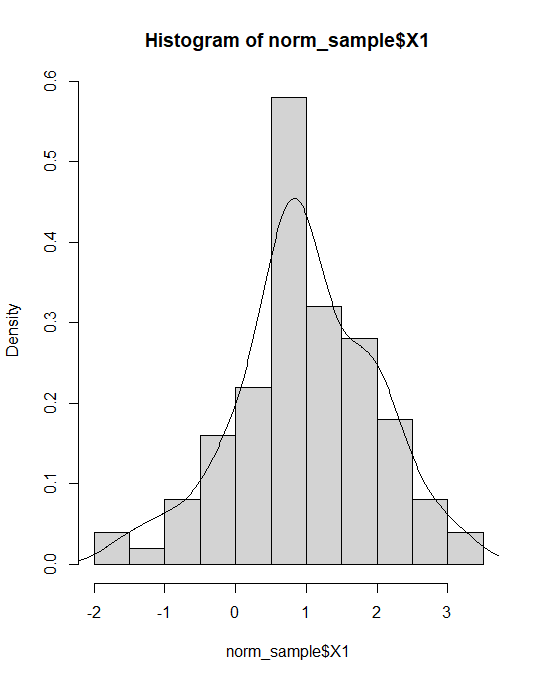
\includegraphics[height=6cm]{Density}
	\end{center}
\end{frame}

\begin{frame}[fragile]{Barplot}
	\begin{itemize}
		\item \verb+ barplot(Spalte1 ~ Spalte2, data) +
	\end{itemize}
			
	\begin{center}
		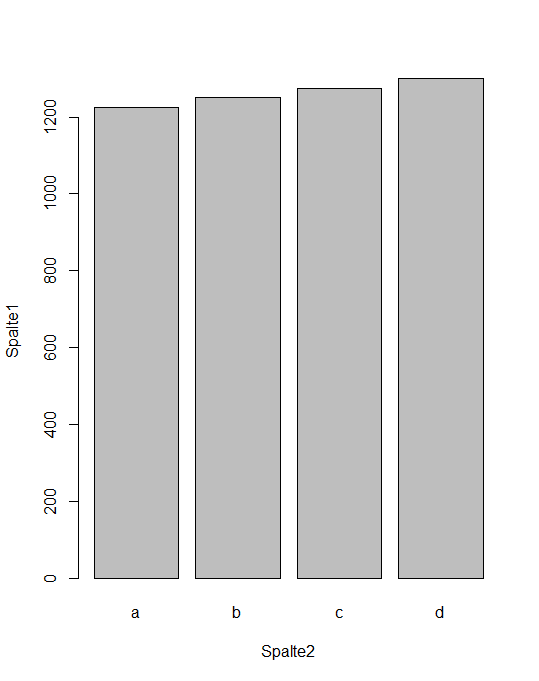
\includegraphics[height=6.5cm]{Barplot}
	\end{center}
\end{frame}

\begin{frame}[fragile]{Speichern von Plots}
	\begin{columns}[T]
		\begin{column}{0.5\textwidth}
			\begin{center}
				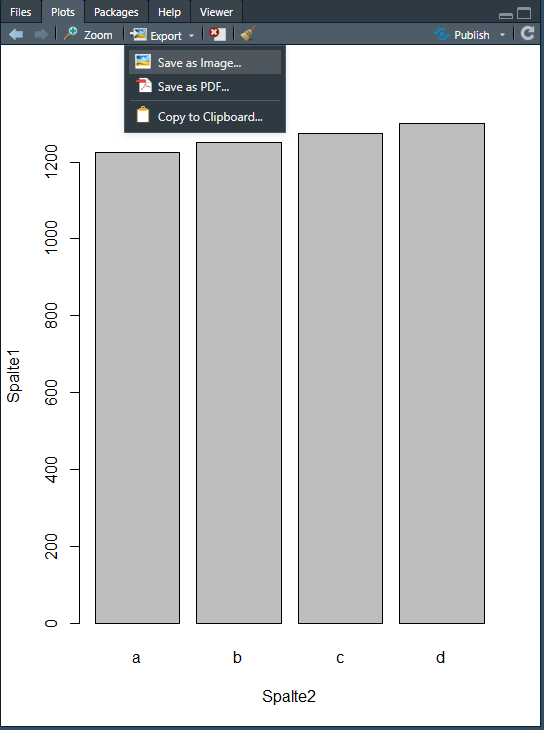
\includegraphics[height=5.5cm]{SaveImage}
			\end{center}
		\end{column}
		\begin{column}{0.5\textwidth}
			\begin{center}
				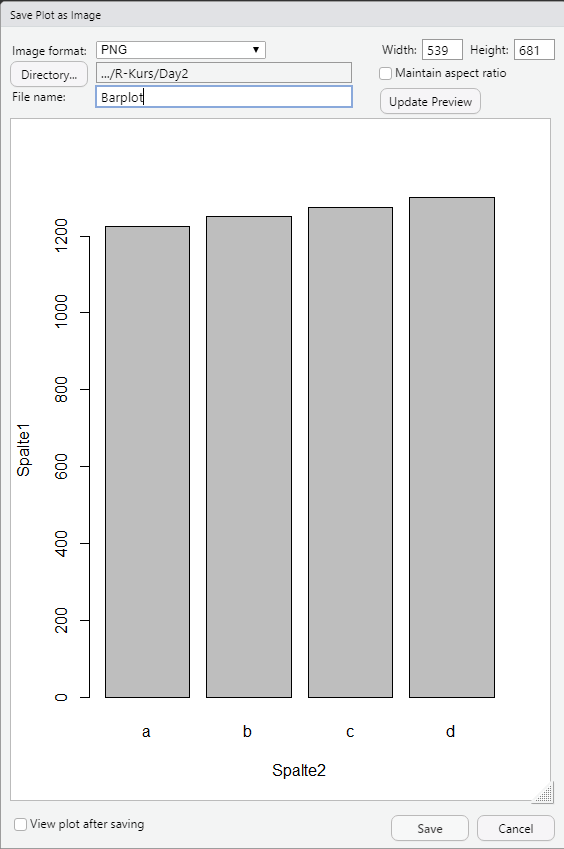
\includegraphics[height=5.5cm]{SaveImage2}
			\end{center}
		\end{column}
	\end{columns}	
\end{frame}

\end{document}
%% ================================================================== %%
%% ================================================================== %% 
